\documentclass{article}
\title{A Partial Comparison Between 52-Week High Method and Industry Momentum Method}
\author{Yolanda Zhao and Ziqi Lu}
\date{January 28, 2015}

\usepackage{Sweave}
\begin{document}
\Sconcordance{concordance:Masterpiece.tex:Masterpiece.Rnw:%
1 5 1 1 0 86 1 1 26 1 3 20 1}

\maketitle

\footnotetext {The data used in this paper is given by Professor David Kane in Kane Capital Management. The code used to generate all the results is available on github, under the repository "l1994z1116q3/Masterpiece." The paper is produced for Economics 20 in the 2015 winter study at Williams College. A special thank to Professor David Kane, the professor in the class, Yuanchu Dang, the teaching fellow in the class, and all the rest of the class.}

\pagebreak


\section{Abstract}


We partially replicate the comparisons of the 52-week high strategy developed by George and Hwang and two traditional momentum strategies in George and Hwang (2004).We use large cap US stock data from 1998 through 2007 to reproduce the average returns from three different strategies, namely, JT strategy, MG strategy, and GH strategy. Beyond that, we also compare the standard deviations of the monthly returns of those strategies. Our goal is to evaluate which of the three strategy is the most profitable and smooth. Unfortunately, MG strategy earns negative monthly returns (-0.71\% for (6,6) and -0.04\% for (6,12)), JT strategy earns a positive return of 0.07\% only in the (6,12) case and GH strategy earns 0.2\% monthly. The standard deviations of their monthly return ranges from 7.35\% for MG strategy to 9.44\% for JT strategy.

\pagebreak

\section{Introduction}


In this paper, we compare three momentum strategies discussed in George and Hwang (2004).The first strategy, JT's individual stock momentum strategy, forms winner (loser) portfolios based on the past returns of individual stocks. The second strategy, MG's industrial momentum strategy is similar to JT's strategy. The only difference is that JT's strategy forms the portfolios based on not the past returns of individual stocks but value-weighted average return for each industry. Both JT and MG use (6,6) strategies : Each month investors form a portfolio based on past 6-month returns, and hold the position for 6 months. Developed by George and Hwang, the 52-week high strategy forms portfolios based on the ratio of current price to its 52-week high price, that is, $\frac{price_{now}}{price_{highest}}$. George and Hwang believe that when the stock price approaches its highest price in the past 52 weeks, the future returns of the stock tend to be high, and vice versa.

The data we use here is the cap US stocks from 1998 to 2007, given by Professor David Kane in Williams College. We calculate the past stock returns using (6, 6)JT strategy and the past industry returns using (6,6) MG strategy.Then we extend both strategies to (6,12) strategies and form portfolios based on the past 12-month returns. We did this because the 52-week high strategy is based on the past 12-month returns.

The result is that in average, the GH strategy earns the highest monthly return, 0.22\% per month, while the JT strategy with 6 months of observation earns a negative profit of 5.76\% per month. MG strategy earns small negative profit for both cases. All of them have high standard deviations from the 7.35\% of MG strategy to the 9.44\% of JT strategy, so the MG strategy is the least risky one as well as the least profitable one in general, while the GH strategy earns the highest return.



\pagebreak

\section{Data Selection}

The data we use in our reproduction is given by Professor David Kane. This is a large cap data about the stock prices in the US stock market from 1998 to 2007. The first monthly return we calculated is the return in January, 2000. Since the last portfolio is formed 6 months ago and a portfolio is formed based on the data of past either 6 or 12 months, the earliest data we use was collected in July 1998. 

We filter the data based on two standards. First, we only study the companies within top 1500 from 2000 to 2007. In each portfolio, we only consider the companies that are in top 1500 when the portfolio is formed, regardless of the past performance of those companies. Therefore, our result suits the top 1500 companies better than the entire US stock market. Second, we only consider the stock returns that are between -200\% and 200\%. Hence we can eliminate abnormal returns, which would skew the average monthly returns of a specific strategy.


\section {Methods}


JT strategy calculates the cumulative return of individual stock. At the end of every month, the strategy calculates the cumulative return of every stock in the past several months and ranks stocks according to their cumulative return. The top 30\% of the stock with high cumulative return in the past are expected to perform well and classified as "winners." The opposite 30\% of the stocks are "losers." The strategy is to buy winners and short losers for 6 months. 

The same method is employed for the MG strategy, except that MG strategy targets at cumulative industry returns instead of individual stock returns. 

The 52-week high strategy uses the data of the past 52 weeks, which we simplify as a whole year. We compare the current price of the stock to its highest price in the past year and rank the stocks based on the ratio of current price to the 52-week high. Then we form our winner (loser) portfolio of the top (bottom) 13\% of stocks with the highest (lowest) ratio of current price to the 52-week high. 

At the end of each month, for each strategy we create a portfolio that selects the stocks based on the data of past 6 or 12 months, and each portfolio will be held for 6 months. When we calculate the returns of a strategy in a single month, we look at the 6 portfolios operating at the same time because we create a new portfolio every month and each of the portfolios are held for 6 months. Finally, we calculate the average return of each of the three strategies from 2000 to 2007 and compare the returns of those strategies to see which one can earn a higher return. Along with the average returns, we calculate the standard deviation of the monthly returns of each strategy. 

\pagebreak

\section{Results}


Table 1 shows the average monthly returns of all three strategies and the variations of JT and MG strategies. The left column represents the names of the strategies and the months of data the strategies investigate. GH strategy always look at 12 months of data, so it is not specified. The second column represents the average monthly return of each individual strategy, and the third column represents the standard deviation of each strategy.


\begin{center}
Table 1: Means and Standard Deviations of The Return of Momentum Strategies
\small This table is a partial replication of GH's table I on page 2148. except that we already combine the winner and loser returns and add standard deviation of monthly return. The data we used is as specified before. 

\begin{table}[ht]
    \centering
    \begin{tabular}{rlrr}
 \hline
 & X & means & sds \\ 
  \hline
1 & Monthly\_JT 6 & -5.76\% & 8.80\% \\ 
  2 & Monthly\_JT12 & 0.75\% & 9.44\% \\ 
  3 & Monthly\_MG6 & -0.71\% & 7.35\% \\ 
  4 & Monthly\_MG12 & -0.04\% & 8.62\% \\ 
  5 & Monthly\_GH & 0.22\% & 8.65\% \\ 
   \hline
\end{tabular}
\caption{Return For Momentum Strategy} 
\end{table}

\end{center}

It turns out that the average monthly returns of all three strategies, including the extension of JT and MG strategies to 12 months, are small or even below 0\%. JT strategy earns positive return of 0.07\% only when its analysis is extended to 12 months, and MG strategy always earns negative return. GH strategy performs the best with a monthly return of 0.215\%, which adds up to 2.4\% every year in average. However, the US inflation calculator shows that the inflation rates between 1999 and 2007 are around or above 3\%, so the GH strategy cannot even beat the inflation for most of the time, and a better investment strategy is to save your money in a bank.

All of the three strategies have high standard deviation, which is at least ten times larger than the average monthly return. In other words, all three strategies are risky and not worth investing. Comparatively, the MG strategy performs the best in terms of risks because its standard deviation is 7.35\% for the 6 months strategy. The 12 month JT strategy has the highest standard deviation of 9.44\%, around 135 times as large as its monthly return.

This table also shows that when we extend the data we use for each portfolio from 6 months to 12 months, the standard deviation of monthly return increases. The standard deviation of JT strategy increases from 8.80\% to 9.44\%, and that of MG strategy increases from 7.35\% to 7.62\%. While the risks increase, the average return also increases as we look at more data for each portfolio. The monthly return of JT strategy increases from -0.576\% to 0.075\%, and the return of MG strategy increases from -0.717\% to -0.042\%. 

Figure 1 is a set of graphs that reflect the monthly return of each of the strategies and their extensions. We can visualize the data for each of them and get an intuition about what is happening.

\begin{center}

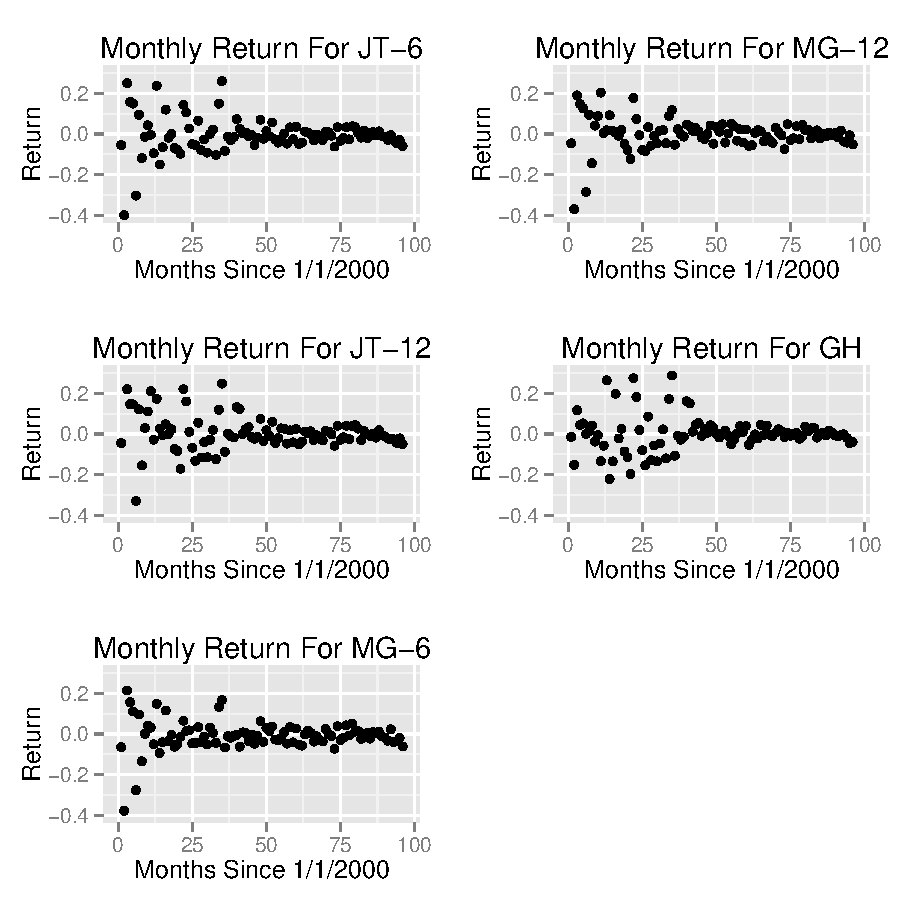
\includegraphics{Masterpiece-001}

\small The graphs here are produced based on the monthly return of all three strategies based on the data from 1998 to 2007. The data is given by Professor David Kane in Williams College.

\end{center}

From the graph, we can see that the monthly return of all those strategies fluctuates strongly after 2000. The fluctuation comes from the Asian Financial Crisis, because stock prices are unstable at that time. Comparatively, the monthly return of the MG strategy recovers faster from the fluctuation while the other two recover slower, so the MG strategy is more resistant to disturbance in the financial market as a whole. The JT and GH strategies, on the other hand, are subject to such fluctuations for longer time.

The other point is that when we apply JT and MG strategies based on past 12 months of performance instead of 6 months, the standard deviation increases and they are subject to loger affect of the financial crisis. Besides the increment of return, the standard deviation for the JT strategy increases from 8.80\% to 9.44\%, and the standard deviation for the MG strategy increases from 7.35\% to 7.62\%. 
 
\section{Conclusion}                       
                                           
The paper compares the three momentum strategies in the paper "52 Week High and Momentum" Investing writen by George and Hwang (2004). The first strategy is called JT strategy. This strategy looks at the daily return of individual stock. The stock with higher cumulative return in the past 6 months is better, and we will buy the stocks with high cumulative return and short the stocks with lower cumulative return. The second strategy is called MG strategy, and the strategy looks at individual industry as a whole instead of individual stock. The third strategy is called GH strategy, and this strategy looks at the ratio of current price to its 52-week high price. We will then buy long the stocks with high price ratio and sell short the stocks with low ratio.                
                      
The data we use is the large cap data of US stock market from 1998 to 2007, given by Professor David Kane. We only look at the data of the top 1500 companies and exclude the daily returns that are larger than 200\%. For each portfolio in JT and MG, we first look at the past returns for 6 months, and then we extend the time to 12 months. 

We replicate a part of the paper, and also consider the standard deviation of monthly returns. The result is that the GH strategy earns the highest monthly profit of 0.22\%, while the MG strategy earns negative profit for both durations of observations. The standard deviation of the return of MG strategy is the least, so the MG strategy is the least risky, while the JT strategy has the highest standard deviation. When we look at the past 12 months of data for both JT and MG strategy, their average monthly returns increase, while their standard deviations also increase and lead to higher risks.


\end{document}


